\documentclass{article}
\usepackage[utf8]{inputenc}
\usepackage{graphicx}
\usepackage{amsmath}
\usepackage{listings}

\title{Oblig 1b: Terningdropp Analysis}
\author{Your Name}
\date{Date of Submission}

\begin{document}

\maketitle

\section{Introduction}
Briefly describe the objective of the assignment and the methods used.

\section{Assignment Questions}

\subsection{Question 2a: First 5 Measurements Regression}
\begin{lstlisting}[language=R]
# Linear Regression on the first 5 measurements in R
lm_first5 <- lm(Lengde ~ Dropp, data=df[1:5, ])
\end{lstlisting}
\textbf{Calculated Regression Line:} Include your manual calculation or calculator output here.

\subsection{Question 2b: Scatter Plot of Data Points}
\textit{Scatter plot of the Dropp vs Lengde data (placeholder image).}
\begin{figure}[h]
    \centering
    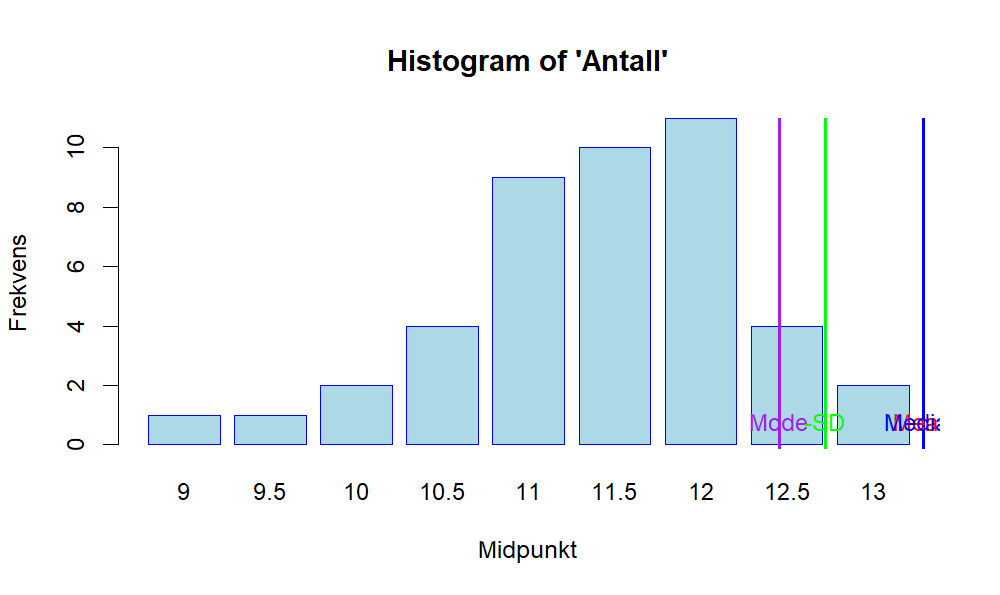
\includegraphics[width=0.8\textwidth]{Rplot02.png}
    \caption{Scatter plot of Dropp vs Lengde}
\end{figure}

\subsection{Question 2c: Regression Line Plot}
\textit{Scatter plot with regression line (placeholder image).}
\begin{figure}[h]
    \centering
    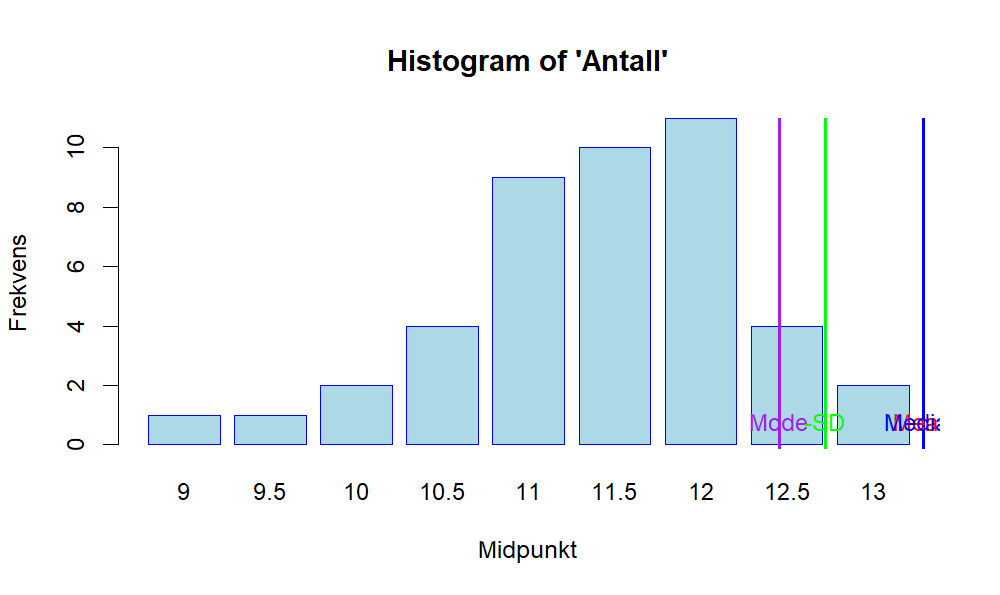
\includegraphics[width=0.8\textwidth]{Rplot02.png}
    \caption{Scatter plot with regression line}
\end{figure}

\subsection{Question 2d: Regression Analysis Entire Dataset}
\begin{lstlisting}[language=R]
# Linear Regression on the entire dataset in R
lm_full <- lm(Lengde ~ Dropp, data=df)
\end{lstlisting}

\subsection{Question 2e: Sum of Squared Residuals (SSe)}
\subsubsection{First 5 Measurements}
\begin{lstlisting}[language=R]
ssr_first5 <- sum(residuals(lm_first5)^2)
\end{lstlisting}
\textbf{SSR for First 5 Measurements:} \[ SSR = <calculated\_value> \]

\subsubsection{Entire Dataset}
\begin{lstlisting}[language=R]
ssr_full <- sum(residuals(lm_full)^2)
\end{lstlisting}
\textbf{SSR for Entire Dataset:} \[ SSR = <calculated\_value> \]

\subsection{Question 2f: Standard Error (se)}
\subsubsection{First 5 Measurements}
\begin{lstlisting}[language=R]
se_first5 <- sqrt(ssr_first5 / lm_first5$df.residual)
\end{lstlisting}
\textbf{Standard Error for First 5 Measurements:} \[ SE = <calculated\_value> \]

\subsubsection{Entire Dataset}
\begin{lstlisting}[language=R]
se_full <- sqrt(ssr_full / lm_full$df.residual)
\end{lstlisting}
\textbf{Standard Error for Entire Dataset:} \[ SE = <calculated\_value> \]

\section{Conclusion}
Summarize your findings and observations from the assignment.

\end{document}
